\documentclass[12pt]{article}

\usepackage{graphicx}
\usepackage{paralist}
\usepackage{listings}
\usepackage{booktabs}
\usepackage{hyperref}
\usepackage{subfig}
\usepackage{float}
\usepackage{mathtools}
\usepackage{fancyvrb}

\lstset{
basicstyle=\small\ttfamily,
columns=flexible,
breaklines=true
}
\DeclarePairedDelimiter\ceil{\lceil}{\rceil}
\DeclarePairedDelimiter\floor{\lfloor}{\rfloor}
\oddsidemargin 0mm
\evensidemargin 0mm
\textwidth 160mm
\textheight 200mm

\pagestyle {plain}
\pagenumbering{arabic}

\newcounter{stepnum}

\title{CS/SE 2XB3 Lab 5 Report\\Enrolled in CSL02}
\author{
  Wang, Mingzhe\\400316660\\
  \texttt{wangm235@mcmaster.ca}
  \and
  Li, Xing\\400292346\\
  \texttt{li64@mcmaster.ca}
  \and
  Moon, Hyosik\\400295620\\
  \texttt{moonh8@mcmaster.ca}
  }
\date{\today}



\begin{document}
\bibliographystyle{plain}

\maketitle

\tableofcontents
\newpage

\section{Implementing Insert}
We implemented the three functions only (\verb|rotate_left()|, \verb|rotate_right()|, and \verb|fix()| ) as provided by the professor. No any other codes are modified.  We tested the algorithm with multiple data sets to cover all possible rotations. The example below is the one to test the extreme of right leaning by inserting the number from 1 to 9, and we compared the result (Figure \ref{r2}) with the expected result (Figure \ref{r1}) as demonstrated at \url{https://www.cs.usfca.edu/~galles/visualization/}.  They are exactly the same, so we are sure our algorithm is correct. 

\begin{figure}[hbt!]
  \centering
  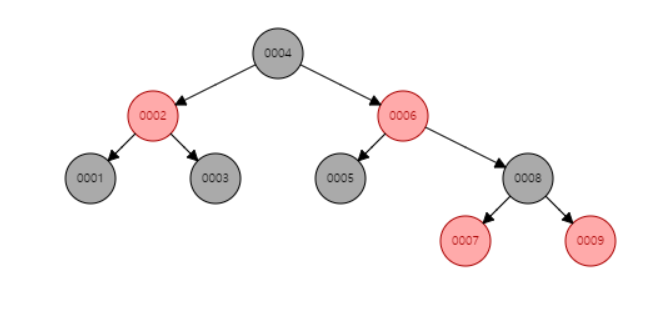
\includegraphics[width=0.5\textwidth]{Figures/RBT3.png}
  \caption{RBT insert result (1 to 9)}
   \label{r1}
\end{figure}

\begin{figure}[hbt!]
  \centering
  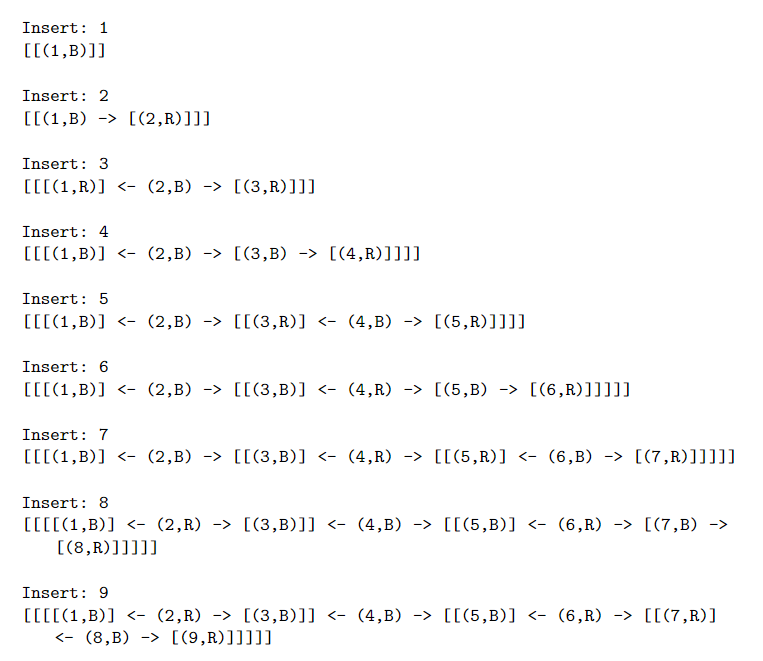
\includegraphics[width=0.6\textwidth]{Figures/r2.png}
  \caption{Python implementation result}
   \label{r2}
\end{figure}

\newpage

\bigskip

\section{Red-Black Tree Height}
\subsection{Insert the numbers from 1 to 10,000}
When we repeated inserting the numbers 1 to 10,000, every time the height of the result was 24. We tested more than 20 times, but the height was always 24. If the implementation is correct, and the order of inserted number is not changed, then the height of the RBT tree should be always the same. This is because the construction of a RBT is constrained by its specific rules, such as ``Red nodes cannot have red children.'', ``All simple paths from the root to a leaf must contain the same number of black nodes.'' . As mentioned in the question. 
However, if the implementation is incorrect, for example, if the root is not reset properly, the height could be wrong.  In our implementation, we knew that after node.parent.parent is rotated, the root might be changed. We added a checker to reset the root accordingly.  Because there are many ways to implement RBT tree,  it's hard to guess the exact reason of the height change. We need to analyze the exception specifically to identify the root cause.

\subsection{Average heights between BSTs and RBTs}
% What is the average difference in the height between the two?
We ran the test to know the average heights of insertion between RBTs and BSTs. Figure \ref{r4} represents the each result of inserting 10,000 randomized elements to RBTs and BSTs. We ran the test 50 times, and the average height is 16.14 for RBTs, and 31.6 for BSTs. The result shows that the RBTs's height is approximately half of BST's height. 

% Comment when we prefer a BST over RBT
~\newline\noindent We tested further to know the trend between the number of elements and height. When we inserted 50,000 and 100,000 (10times, 5times respectively), it showed that the average length of RBTs 19.1, 20.0 and 38.3, 40.6 for BSTs respectively. With the results, we know that the hight of RBTs is approximately half of the BSTs. This big difference between the two trees are shown in Figure \ref{r5}. So, we can simply know that the time complexity of RBTs will be better than BSTs when searching an item in the tree. However, if in a specific scenario, there are very few searching and many insertions, the additional cost of rebalancing RBT might not be paid off by the gain from searching. In that case, BST would be preferred over an RBT.


\begin{figure}[hbt!]
  \centering
  \subfloat[Height of insertion (10,000(n), 50times)]{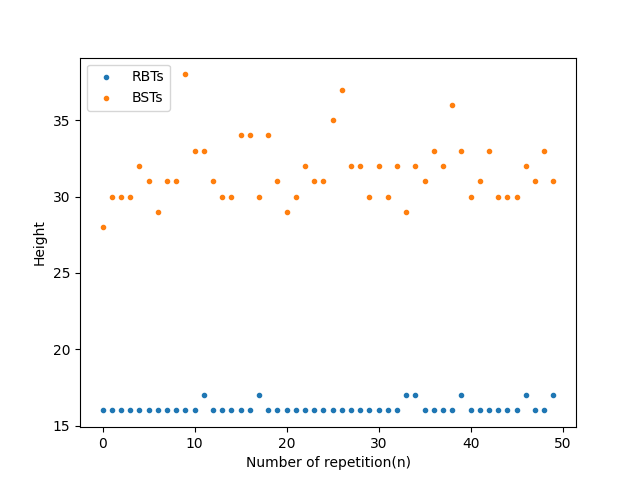
\includegraphics[width=0.49\textwidth]{Figures/rbt_bst_avg_10000.png}\label{r4}}
  \hfill
  \subfloat[Height of insertion (50,000(n), 10times)]{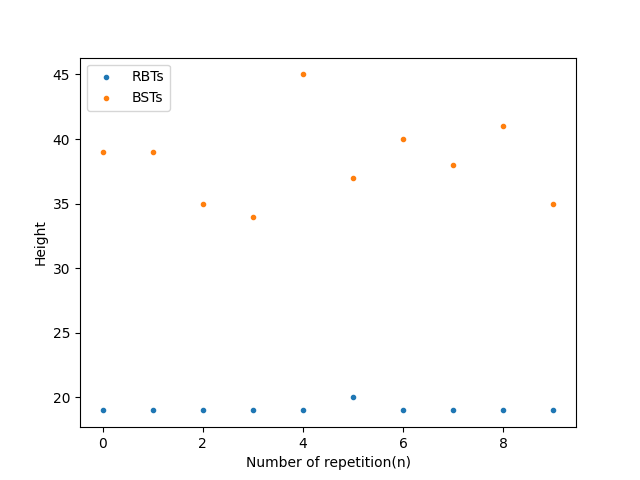
\includegraphics[width=0.49\textwidth]{Figures/rbt_bst_avg_50000.png}\label{r5}}
  \caption{Red Black Tree insert result}
\end{figure}

\newpage 

\subsection{Average heights between BSTs and RBTs for sorted input}
%  Graph the height of a BST and RBT vs the near sorted factor of the list. What do you observe?

\begin{figure}[hbt!]
  \centering
  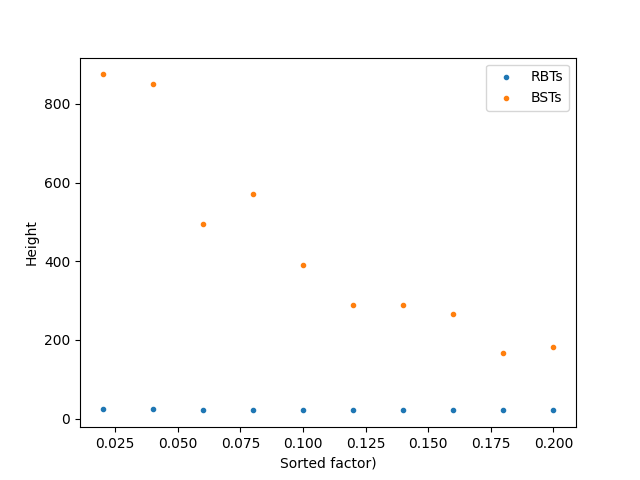
\includegraphics[width=0.5\textwidth]{Figures/sorted_case.png}
  \caption{Heights of RBTs and BSTs (sorted lists)}
   \label{r6}
\end{figure}

We tested the average heights of BSTs and RBTs based on sorted lists. We ran the test changing the factor from 0.02 to 0.20. The main observations are listed below:
\begin{itemize}
\item The average heights of the trees were 22.6 for RBTs and 437.7 for BSTs. 
\item As the number of sorted items in the list increases, the BSTs' performance becomes worse, while the RBTs' performance almost remains the same. 
\item We can induce that in the worst case, when the list is totally sorted, the height of the BSTs will be nearly 10000, which is the length of the list.
\end{itemize}



\begin{thebibliography}{9}
\bibitem{codesdope} 
Red Black Tree,\\
\texttt{https://www.codesdope.com/course/data-structures-red-black-trees-insertion/}

% \bibitem{wikipedia} 
% Binary heap,\\
% \texttt{https://en.wikipedia.org/wiki/Binary\_heap}

% \bibitem{wikipedia2} 
% k-ary heap,\\
% \texttt{https://en.wikipedia.org/wiki/D-ary\_heap}

% \bibitem{Geeks}
% m-ary tree,\\
% \texttt{https://www.quora.com/What-are-advantages-of-using-a-d-ary-tree-instead\\-of-a-binary-tree}

\end{thebibliography}

\end{document}
